\documentclass[10pt,a4paper,landscape]{article}
\usepackage[margin=0.5cm]{geometry}
\usepackage[utf8]{inputenc}
\usepackage[T1]{fontenc}
\usepackage[english]{babel}
\usepackage{multicol}
\usepackage{booktabs}
\usepackage{tabularx}
\usepackage{array}
\usepackage{xcolor}
\usepackage{tcolorbox}
\usepackage{enumitem}
\usepackage{tikz}
\usetikzlibrary{positioning,shapes}
\usepackage{fancyhdr}
\usepackage{amsmath}

% Color definitions
\definecolor{darkblue}{RGB}{44,62,80}
\definecolor{orange}{RGB}{243,156,18}
\definecolor{red}{RGB}{231,76,60}
\definecolor{blue}{RGB}{52,152,219}
\definecolor{gray}{RGB}{149,165,166}

% Tcolorbox configuration
\tcbuselibrary{skins,breakable}

% Style for main sections
\newtcolorbox{mainsection}[1]{
	enhanced,
	colback=darkblue!10,
	colframe=red,
	fonttitle=\bfseries\small,
	title=#1,
	boxrule=1pt,
	left=2pt,
	right=2pt,
	top=2pt,
	bottom=2pt
}

% Style for formulas
\newtcolorbox{formula}{
	enhanced,
	colback=red!20,
	colframe=red,
	boxrule=1pt,
	left=3pt,
	right=3pt,
	top=3pt,
	bottom=3pt
}

% Command for highlighted text
\newcommand{\highlight}[1]{\textcolor{orange}{\textbf{#1}}}
\newcommand{\critical}[1]{\textcolor{red}{\textbf{#1}}}
\newcommand{\info}[1]{\textcolor{blue}{\textbf{#1}}}

% Page configuration
\pagestyle{fancy}
\fancyhf{}
\fancyhead[C]{\Large\textbf{\textcolor{red}{🗡️ COMBAT SUMMARY SHEET - OBSS 🗡️}}}
\renewcommand{\headrulewidth}{2pt}
\renewcommand{\headrule}{\hbox to\headwidth{\color{red}\leaders\hrule height \headrulewidth\hfill}}

\setlength{\parindent}{0pt}
\setlength{\parskip}{2pt}
\setlength{\columnsep}{8pt}

\begin{document}
	
	\begin{multicols}{4}
		
		% COMBAT SEQUENCE
		\begin{mainsection}{📋 COMBAT SEQUENCE}
			\begin{center}
				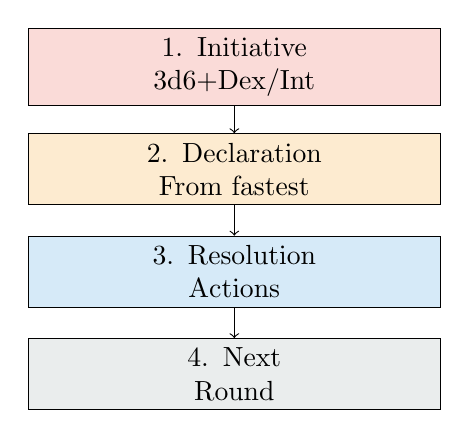
\begin{tikzpicture}[node distance=1.3cm, auto]
					\node[draw, rectangle, fill=red!20, text width=5cm, text centered, font=\normalsize] (init) {1. Initiative\\3d6+Dex/Int};
					\node[draw, rectangle, fill=orange!20, text width=5cm, text centered, font=\normalsize, below of=init] (decl) {2. Declaration\\From fastest};
					\node[draw, rectangle, fill=blue!20, text width=5cm, text centered, font=\normalsize, below of=decl] (res) {3. Resolution\\Actions};
					\node[draw, rectangle, fill=gray!20, text width=5cm, text centered, font=\normalsize, below of=res] (next) {4. Next\\Round};
					
					\draw[->] (init) -- (decl);
					\draw[->] (decl) -- (res);
					\draw[->] (res) -- (next);
				\end{tikzpicture}
			\end{center}
			
			\textbf{Critical Initiative:}
			\begin{itemize}[noitemsep,leftmargin=8pt]
				\item If +8: +1 Reaction/Immediate
				\item If +16: +1 total Action
			\end{itemize}
		\end{mainsection}
		
		% ACTIONS PER ROUND
		\begin{mainsection}{⚡ ACTIONS PER ROUND}
			\begin{formula}
				\textbf{Available each round:}\\
				• 3 Normal Actions\\
				• 1 Immediate Action\\
				• 1 Reaction Action\\
				• Unlimited Free Actions
			\end{formula}
			
			\textbf{Action Order:} Any, logically coherent
			
			\textbf{Interruptions:} Only Reactions and Immediate can interrupt
		\end{mainsection}
		
		% ATTACK ROLLS
		\begin{mainsection}{🎯 ATTACK ROLLS}
			\begin{formula}
				\textbf{Melee:}\\
				3d6 + BAB + STR + List + Skill + Magic + Circumstances
			\end{formula}
			
			\begin{formula}
				\textbf{Ranged:}\\
				3d6 + BAB + DEX + List + Skill + Magic + Circumstances
			\end{formula}
			
			\textbf{Golden Rules:}
			\begin{itemize}[noitemsep,leftmargin=8pt]
				\item \highlight{6 = Explodes} (roll again)
				\item \critical{1 = Counts as 0}
				\item \highlight{Trust to luck:} -4 for +1d6
				\item \critical{3 times 1 = Automatic miss}
				\item \highlight{3 times 6 = Always hits}
			\end{itemize}
		\end{mainsection}
		
		% DEFENSE
		\begin{mainsection}{🛡️ DEFENSE}
			\begin{formula}
				10 + DEX + Shield + Armor + Magic + Skill + Circumstances
			\end{formula}
			
			\begin{tabular}{@{}ll@{}}
				\toprule
				\textbf{Situation} & \textbf{Modifier} \\
				\midrule
				Surprised & -2 Defense \\
				Prone & -4 Defense \\
				Fatigued (1/2/3) & -1/-2/-4 \\
				Grappled & -2 Defense \\
				Entangled & -2 Defense \\
				Pinned & -4 Defense \\
				Stunned & -4 Defense \\
				Cover L/M/C & +2/+4/+8 \\
				\bottomrule
			\end{tabular}
		\end{mainsection}
		
		\columnbreak
		
		% DAMAGE AND CRITICALS
		\begin{mainsection}{💥 DAMAGE AND CRITICALS}
			\begin{formula}
				\textbf{Base Damage:}\\
				Weapon Die + STR + List + Skill + Magic
			\end{formula}
			
			\textbf{Critical Roll:}
			\begin{itemize}[noitemsep,leftmargin=8pt]
				\item \critical{Each +8 beyond Defense} = +1 Critical
				\item Roll additional weapon die (base die only)
				\item Does not stack with damage explosion
			\end{itemize}
			
			\textbf{Damage Explosion:}
			\begin{itemize}[noitemsep,leftmargin=8pt]
				\item Maximum die value: Reroll and add
				\item Does not explode on: Criticals, dice <=d6
				\item EDX: Explodes on X or higher
				\item Does not explode recursively
			\end{itemize}
			
			\textbf{Minimum Damage:} Always at least 1 (after reductions)
		\end{mainsection}
		
		% MULTIPLE ATTACKS
		\begin{mainsection}{⚔️ MULTIPLE ATTACKS}
			\begin{tabular}{@{}cc@{}}
				\toprule
				\textbf{Attack} & \textbf{Penalty} \\
				\midrule
				1 & +0 \\
				2 & -5 \\
				3 & -10 \\
				4 & -15 \\
				\bottomrule
			\end{tabular}
			
			\textbf{Two Weapons:}
			\begin{itemize}[noitemsep,leftmargin=8pt]
				\item Off-hand weapon = Multiple attack
				\item STR halved on off-hand
				\item If not Light: \critical{-3 additional}
				\item Can use for +1 Defense (no attacks)
			\end{itemize}
			
			\textbf{Low Level Option:}\\
			BAB < 6: -4 on both instead of progression
		\end{mainsection}
		
		% MOVEMENT
		\begin{mainsection}{🏃 MOVEMENT AND DISTANCES}
			\begin{tabular}{@{}p{2cm}p{1cm}p{2.5cm}@{}}
				\toprule
				\textbf{Type} & \textbf{Cost} & \textbf{Distance} \\
				\midrule
				Normal & 1 Act. & Base move \\
				Run & 1 Act. & 2x Move \\
				Diff. Terr. & - & 1/2 Move \\
				Diagonal & - & 1m/square \\
				\bottomrule
			\end{tabular}
			
			\textbf{Running Penalties:}
			\begin{itemize}[noitemsep,leftmargin=8pt]
				\item \critical{-1d6 Attack Roll}
				\item \critical{-4 Defense} (until next round)
				\item Distracted for spells
			\end{itemize}
			
			\textbf{Distances:}
			\begin{itemize}[noitemsep,leftmargin=8pt]
				\item \textbf{Touch:} ≤ 1m (without long weapons)
				\item \textbf{Melee:} ≤ 1m (2m with long weapons)
				\item \textbf{Reach:} Half Size occupied
			\end{itemize}
		\end{mainsection}
		
		\columnbreak
		
		% MAIN ACTIONS
		\begin{mainsection}{📜 MAIN ACTIONS}
			{\small
				\begin{tabular}{@{}p{2cm}cp{3cm}@{}}
					\toprule
					\textbf{Action} & \textbf{Act.} & \textbf{Notes} \\
					\midrule
					Single attack & 1 & One Attack Roll \\
					Two attacks & 2 & Second at -5 \\
					Three+ attacks & 3 & Cumulative penalties \\
					\midrule
					Movement & 1 & Up to maximum \\
					Run & 1 & 2x mov., penalties \\
					Charge & 2 & Mov.+att., +1d6 AR, -4 Def \\
					\midrule
					Spell & 2* & Varies per spell \\
					Prep. Defense & 1 & +1 Defense \\
					Total Defense & 2 & +4 Def., diff. terrain \\
					Disengage & 1 & 1m without provoking \\
					Precise Strike & 2 & One attack +1d4 AR \\
					\midrule
					Stand from Prone & 1 & Acrobatics DC13 (Imm.) \\
					Draw/Sheathe & 1 & Free with movement \\
					Search Backpack & 2 & - \\
					Take from Belt & 1 & - \\
					\midrule
					Drink Potion & I. & If in hand \\
					Give Drink & 2 & To another \\
					Mount/Dismount & 2 & From mount \\
					\bottomrule
				\end{tabular}
			}
		\end{mainsection}
		
		% SPECIAL MANEUVERS
		\begin{mainsection}{🤺 SPECIAL MANEUVERS}
			\begin{tabular}{@{}p{1.7cm}p{0.8cm}p{3cm}@{}}
				\toprule
				\textbf{Maneuver} & \textbf{Cost} & \textbf{Opposed Check} \\
				\midrule
				Disarm & 2 & BAB+STR/DEX vs BAB+STR/DEX \\
				Feint & 1 & BAB+Bluff vs BAB+Sense \\
				Bull Rush & 2 & Athletics vs Fort ST+STR \\
				Grapple & 2 & Athletics vs Fort ST+STR \\
				Trip & 2 & Athletics vs Fort ST+STR \\
				Overrun & 1 & Athl/Acrob. vs Ref ST \\
				\bottomrule
			\end{tabular}
			
			\textbf{Size Modifiers:}
			\begin{itemize}[noitemsep,leftmargin=8pt]
				\item +1d6 per size advantage
				\item -1d6 per size disadvantage
			\end{itemize}
			
			\textbf{Critical Failure:} You suffer the effect
		\end{mainsection}
		
		% RANGED WEAPONS
		\begin{mainsection}{🏹 RANGED WEAPONS}
			\begin{tabular}{@{}lc@{}}
				\toprule
				\textbf{Increment} & \textbf{AR Penalty} \\
				\midrule
				1st (within range) & +0 \\
				2nd (range × 2) & -6 \\
				3rd (range × 3) & -12 \\
				\bottomrule
			\end{tabular}
			\medskip
			\textbf{Under Threat:} -1d6 AR for ranged weapons
			
			\textbf{Against Target in Combat:}
			\begin{itemize}[noitemsep,leftmargin=8pt]
				\item -2 additional AR
				\item Cover from other creatures
				\item Critical failure: hit randomly
			\end{itemize}
			
			\textbf{Strength to Damage:}
			\begin{itemize}[noitemsep,leftmargin=8pt]
				\item Composite bows: Yes
				\item Normal bows: No
				\item Crossbows: No
				\item Thrown weapons: Yes
			\end{itemize}
		\end{mainsection}
		
		\columnbreak
		
		% SITUATIONAL MODIFIERS
		\begin{mainsection}{🎲 SITUATIONAL MODIFIERS}
			\textbf{ATTACKER}
			\begin{tabular}{@{}p{3.5cm}c@{}}
				\toprule
				\textbf{Situation} & \textbf{Mod} \\
				\midrule
				Flanking & +2 \\
				Higher Ground & +2 \\
				Attack from Behind & +2 \\
				Invisible & +1d6 \\
				Charge & +1d6 \\
				Helpless Opponent & +1d6 \\
				Touch Attack & +1d6 \\
				\midrule
				Prone & -4 \\
				Fatigued (1/2/3) & -1/-2/-3 \\
				Dim Light & -1 \\
				Squeezed & -1d6 \\
				Frightened & -1d6 \\
				Unknown Weapon & -1d6 \\
				Invisible Target & -1d6 \\
				Long Weapon at <2m & -4 \\
				Nonlethal Attack & -4 \\
				\bottomrule
			\end{tabular}
			
			\vspace{2mm}
			
			\textbf{DEFENDER}
			\begin{tabular}{@{}p{3.5cm}c@{}}
				\toprule
				\textbf{Situation} & \textbf{Mod} \\
				\midrule
				Light Cover & +2 \\
				Medium Cover & +4 \\
				Complete Cover & +8 \\
				\midrule
				Surprised & -2 \\
				Prone & -4 \\
				Grappled & -2 \\
				Entangled & -2 \\
				Pinned & -4 \\
				Stunned & -4 \\
				Fatigued (1/2/3) & -1/-2/-3 \\
				\bottomrule
			\end{tabular}
		\end{mainsection}
		
		% CONDITIONS AND STATES
		\begin{mainsection}{😵 COMMON CONDITIONS}
			\begin{tabular}{@{}p{2.2cm}p{3.4cm}@{}}
				\toprule
				\textbf{Condition} & \textbf{Effects} \\
				\midrule
				Prone & -4 AR and Def in melee \\
				Fatigued & -1/-2/-4 to AR and Def \\
				Distracted & Penalized Magic Check \\
				Frightened & -1d6 to actions \\
				Confused & Random actions \\
				Paralyzed & Helpless, immobile \\
				Unconscious & Helpless, incapable \\
				Dying & Negative HP, -1 HP/round \\
				Blinded & Miss chance 50\% \\
				Deafened & -4 Initiative \\
				Nauseated & 1 action max \\
				Entangled & -2 AR, Def, Dex \\
				Grappled & -2 Def, Distracted \\
				Pinned & -4 Def, no movement \\
				\bottomrule
			\end{tabular}
		\end{mainsection}
		
		% LIFE AND DEATH
		\begin{mainsection}{💀 LIFE AND DEATH}
			\begin{formula}
				\textbf{Health States:}\\
				• \highlight{HP > 0}: Normal\\
				• \highlight{HP = 0}: Unconscious\\
				• \critical{HP < 0}: Dying (-1 HP/round)\\
				• \critical{HP <= -(10+CON×2)}: Dead
			\end{formula}
			
			\textbf{Recovery from 0 HP:}
			\begin{itemize}[noitemsep,leftmargin=8pt]
				\item Magical healing = Heal HP
				\item First Aid DC 12 = 1 HP
				\item After 1h: Fort ST DC 15 = 1 HP or -1 HP
			\end{itemize}
			
			\textbf{Recovery from Dying:}
			\begin{itemize}[noitemsep,leftmargin=8pt]
				\item First Aid DC (12+neg HP) = 0 HP
				\item Difficulty +2 per successive attempt
				\item Magical healing = 1 HP
			\end{itemize}
			
			\textbf{Natural Recovery:}
			\begin{itemize}[noitemsep,leftmargin=8pt]
				\item 8h rest: CON×BAB or CON×CL HP
				\item Nonlethal HP: CON HP/hour
				\item Max HP: 1d4+CON per rest
			\end{itemize}
		\end{mainsection}
		
		% QUICK RULES
		\begin{mainsection}{⚡ QUICK RULES}
			\textbf{Long Weapons:} 2m reach, -4 AR under 2m
			
			\textbf{Versatile Weapons:} DEX instead STR for AR
			
			\textbf{Set vs Charge:} Ready vs charge (Reaction), then free attack with -1d6
			
			\medskip
			
			\textbf{Time:}
			\begin{itemize}[noitemsep,leftmargin=8pt]
				\item 1 Round = 10 seconds
				\item 1 Minute = 6 rounds
				\item 1 Turn = 10 minutes
			\end{itemize}
			
			\textbf{Reactivation:} "1/day" items/abilities recharge at dawn
			
			\medskip
			
			\textbf{Mounts:}
			\begin{itemize}[noitemsep,leftmargin=8pt]
				\item 2 Actions, uses your initiative
				\item If hit: Ride DC 15 or dismounted
				\item +2 AR from higher ground
			\end{itemize}
		\end{mainsection}
		
	\end{multicols}
	
	% ATTACK FLOWCHART (bottom section)
	\begin{center}
		\begin{tcolorbox}[enhanced,colback=gray!10,colframe=red,title=🎯 ATTACK RESOLUTION FLOWCHART,fonttitle=\bfseries]
			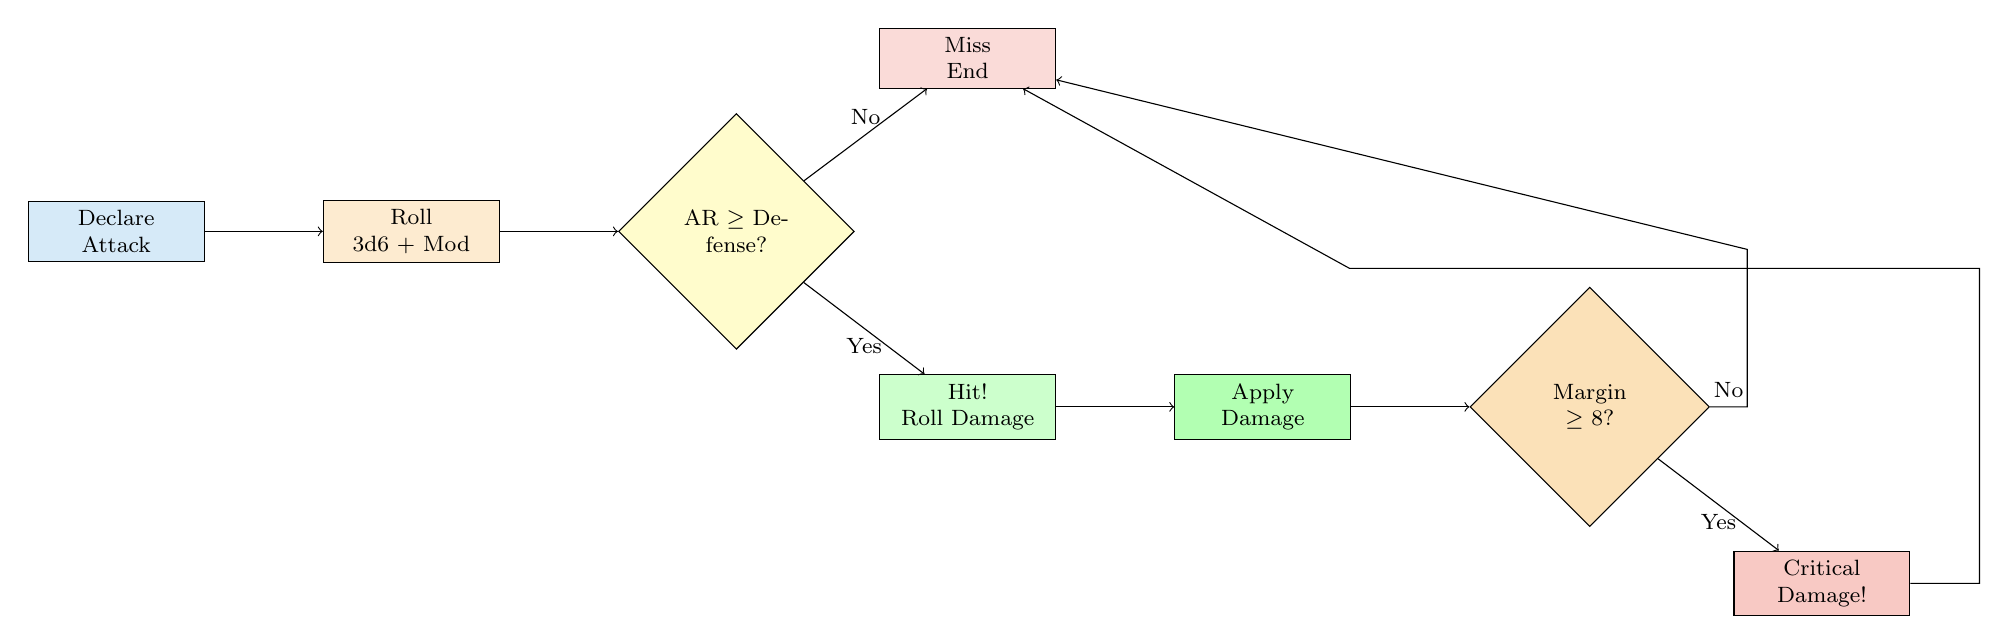
\begin{tikzpicture}[node distance=1.5cm, font=\footnotesize]
				\node[draw, rectangle, fill=blue!20, text width=2cm, align=center] (start) {Declare\\Attack};
				\node[draw, rectangle, fill=orange!20, text width=2cm, align=center, right=of start] (roll) {Roll\\3d6 + Mod};
				\node[draw, diamond, fill=yellow!20, text width=2cm, align=center, right=of roll] (compare) {AR $\geq$ Defense?};
				\node[draw, rectangle, fill=green!20, text width=2cm, align=center, below right=of compare] (hit) {Hit!\\Roll Damage};
				\node[draw, rectangle, fill=red!20, text width=2cm, align=center, above right=of compare] (miss) {Miss\\End};
				\node[draw, rectangle, fill=green!30, text width=2cm, align=center, right=of hit] (damage) {Apply\\Damage};
				\node[draw, diamond, fill=orange!30, text width=2cm, align=center, right=of damage] (crit) {Margin\\$\geq$ 8?};
				\node[draw, rectangle, fill=red!30, text width=2cm, align=center, below right=of crit] (critdmg) {Critical\\Damage!};
				
				\draw[->] (start) -- (roll);
				\draw[->] (roll) -- (compare);
				\draw[->] (compare) -- node[above] {No} (miss);
				\draw[->] (compare) -- node[below] {Yes} (hit);
				\draw[->] (hit) -- (damage);
				\draw[->] (damage) -- (crit);
				\draw[->] (crit) -- node[above] {No} ++(2,0) -- ++(0,2) -- (miss);
				\draw[->] (crit) -- node[below] {Yes} (critdmg);
				\draw[->] (critdmg) -- ++(2,0) -- ++(0,2) -- ++(0,2) -- ++(-8,0) -- (miss);
			\end{tikzpicture}
		\end{tcolorbox}
	\end{center}
	
\end{document}